\documentclass[11pt]{beamer}

\mode<presentation> {
    \usetheme{Madrid}
}

\usepackage{lmodern}
\usepackage{media9}

\usepackage[square,numbers]{natbib}
\usepackage[utf8]{inputenc}
\usepackage{amsmath, amssymb, amsthm}
\usepackage{array}
\usepackage{booktabs}
\usepackage{graphicx}
\usepackage{hhline}
\usepackage{ragged2e}
\usepackage{subcaption}
\usepackage{tabularx, caption}
\usepackage{tabularx,booktabs,ragged2e}
\usepackage{vntex}

\bibliographystyle{ieeetr}
\justifying
\numberwithin{figure}{section}
\numberwithin{table}{section}
\renewcommand{\baselinestretch}{1.1}
\setbeamertemplate{caption}[numbered]

\input{settings/header}
\input{settings/footer}
\usepackage[english]{babel}

\title[Master Thesis Report]{
    Application of Large Language Models in Software Error Debugging
}

\author[Tang Quoc Thai]{
Tang Quoc Thai\\[4mm]
{\small \textit{Instructors} \\[1mm]
Assoc. Prof.\ Quan Thanh Tho \\
Assoc. Prof.\ Huynh Tuong Nguyen}}

\institute[HCMUT]
{VIETNAM NATIONAL UNIVERSITY HO CHI MINH CITY\\
    HO CHI MINH UNIVERSITY OF TECHNOLOGY \\
    \medskip
}

\date{\today}


\newcommand\Wider[2][3em]{
\makebox[\linewidth][c]{
    \begin{minipage}{\dimexpr\textwidth+#1\relax}
    \raggedright#2
    \end{minipage}
    }
}

\begin{document}

\begin{frame}
    \Wider[-1cm]{\titlepage}
\end{frame}

\begin{frame}
    \frametitle{Table of Contents}
    \Wider[-1cm]{\tableofcontents[subsectionstyle = hide, subsubsectionstyle = hide]}
\end{frame}

\AtBeginSection[]
{
    \begin{frame}[plain]
        \frametitle{Table of Contents}
        \Wider[-1cm]{\tableofcontents[sectionstyle=show, subsectionstyle=show/show/hide, subsubsectionstyle=show/show/hide/hide, currentsection, hideothersubsections]}
    \end{frame}
}

% Contents
\section{Introduction}

\begin{frame}{Introduction}
    The rise of Large Language Models (LLMs) is transforming software development. However, their current application primarily relies on zero-shot learning, limiting their ability to tackle complex programming tasks.

    \vspace{0.5cm}

    Can we unlock the full potential of LLMs for sophisticated software development by empowering them with reasoning capabilities and domain-specific knowledge?

    \begin{figure}[!htb]
        \centering
        
\includegraphics[width=0.5\textwidth]{img/llm_for_coding}
    \end{figure}
\end{frame}

\begin{frame}{Introduction}
    This thesis introduces \textbf{CoT-SelfEvolve}, a novel framework that enhances LLMs through:

    \begin{itemize}
        \item \textbf{Chain-of-Thought prompting} to guide LLM reasoning.
        \item \textbf{Integration of external knowledge} from StackOverflow to provide domain-specific context.
    \end{itemize}

    \begin{figure}[!htb]
        \centering
        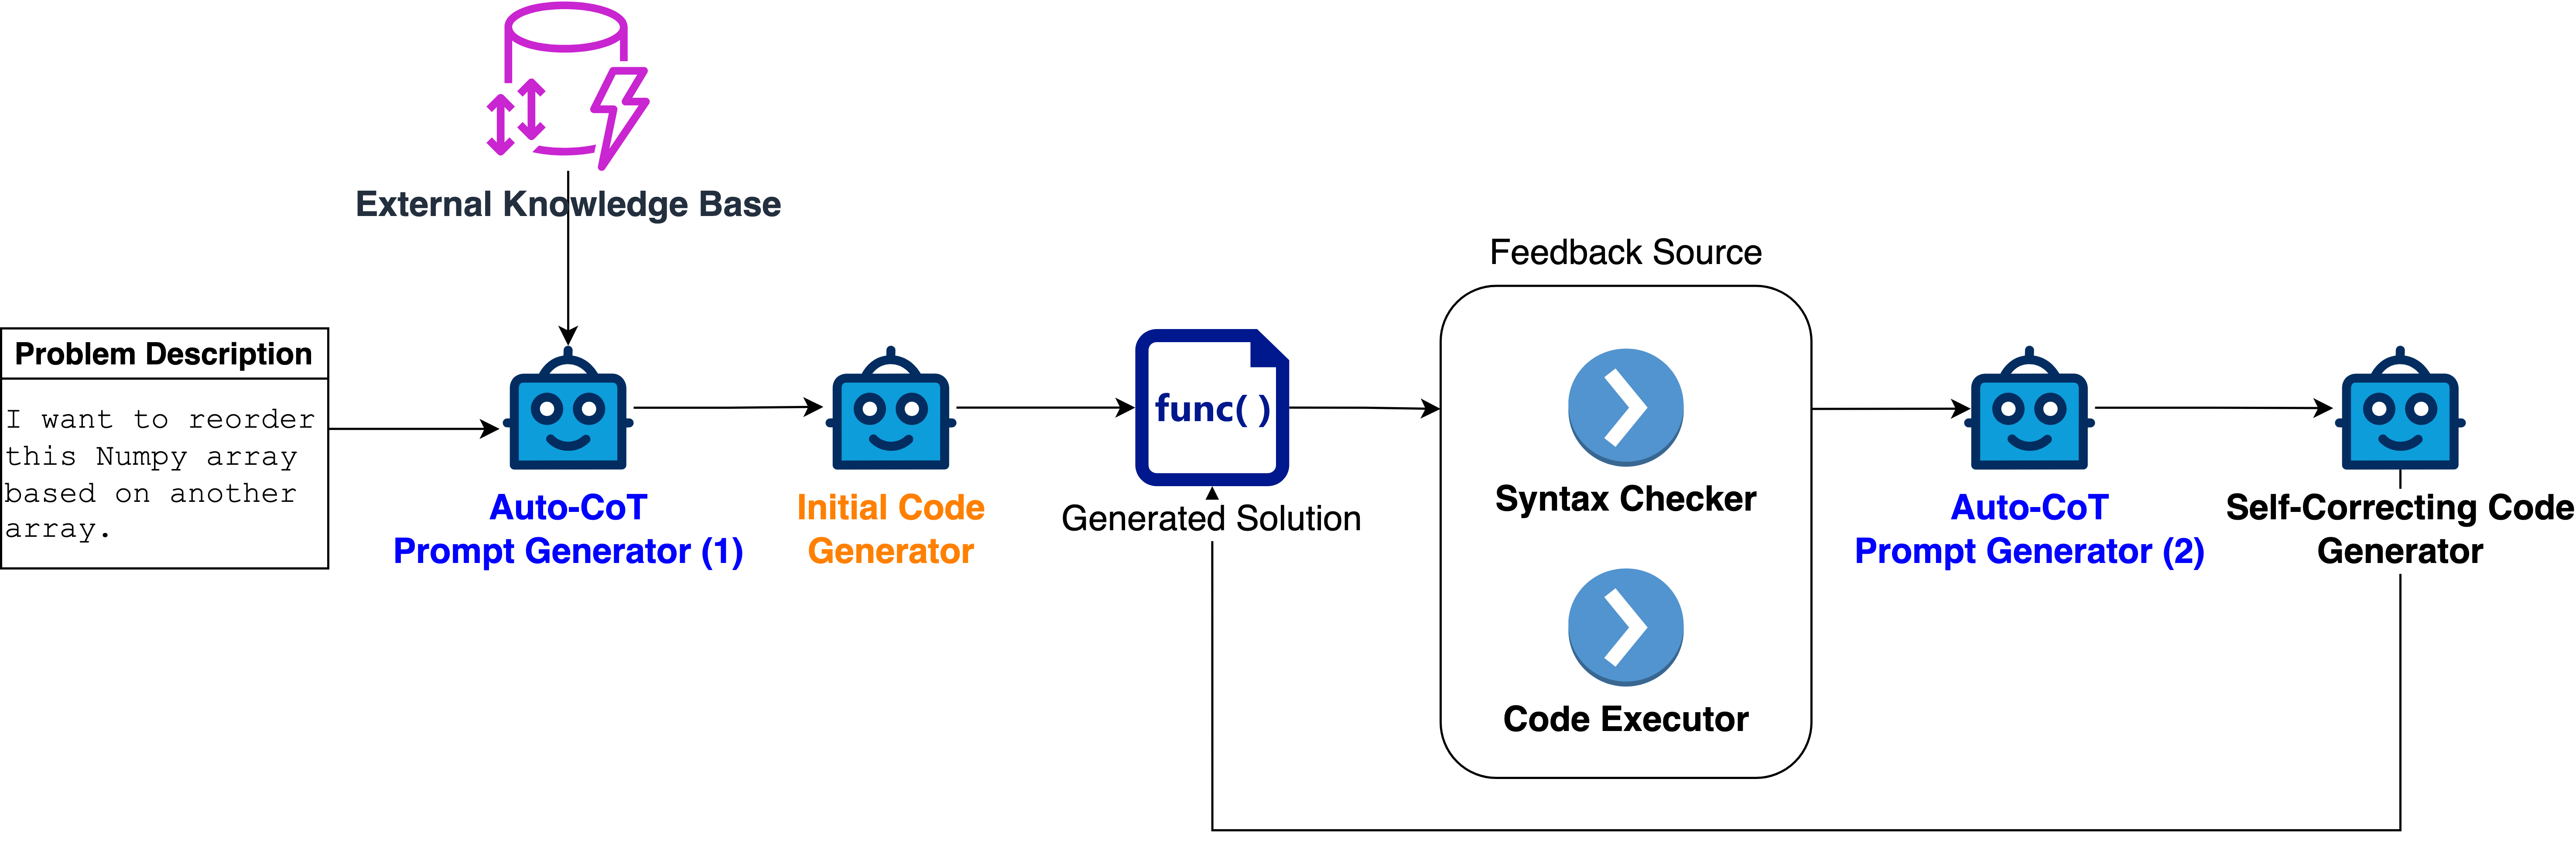
\includegraphics[width=0.8\textwidth]{img/cot_selfevolve_architecture}
        \captionsetup{font=small,labelformat=empty}
        \caption{Architecture of the CoT-SelfEvolve model (this study).}
    \end{figure}
\end{frame}

\section{Related Works}

\begin{frame}{Problem Formulation}
    \begin{block}{Problem}
        Given a set of problems (software bugs) be denoted as \( P = \{P_1, P_2, \ldots, P_N\} \), where each problem \( P_i \) is associated with a description \( D_i \) detailing the observed errors.\\

        Additionally, for each problem \( P_i \), there exist multiple unit tests \( U_{i,j} \) representing different test cases to validate the correctness of the fixed code. The model has access to these unit tests to guide the correction process.\\

        The goal is to maximize the `pass@k' metric, which is defined as the percentage of problems in the set for which the $k$ initial attempts at correction passes all associated unit tests successfully.
    \end{block}
\end{frame}

\begin{frame}{Taxonomy of Related Works}
    \begin{figure}
        \centering
        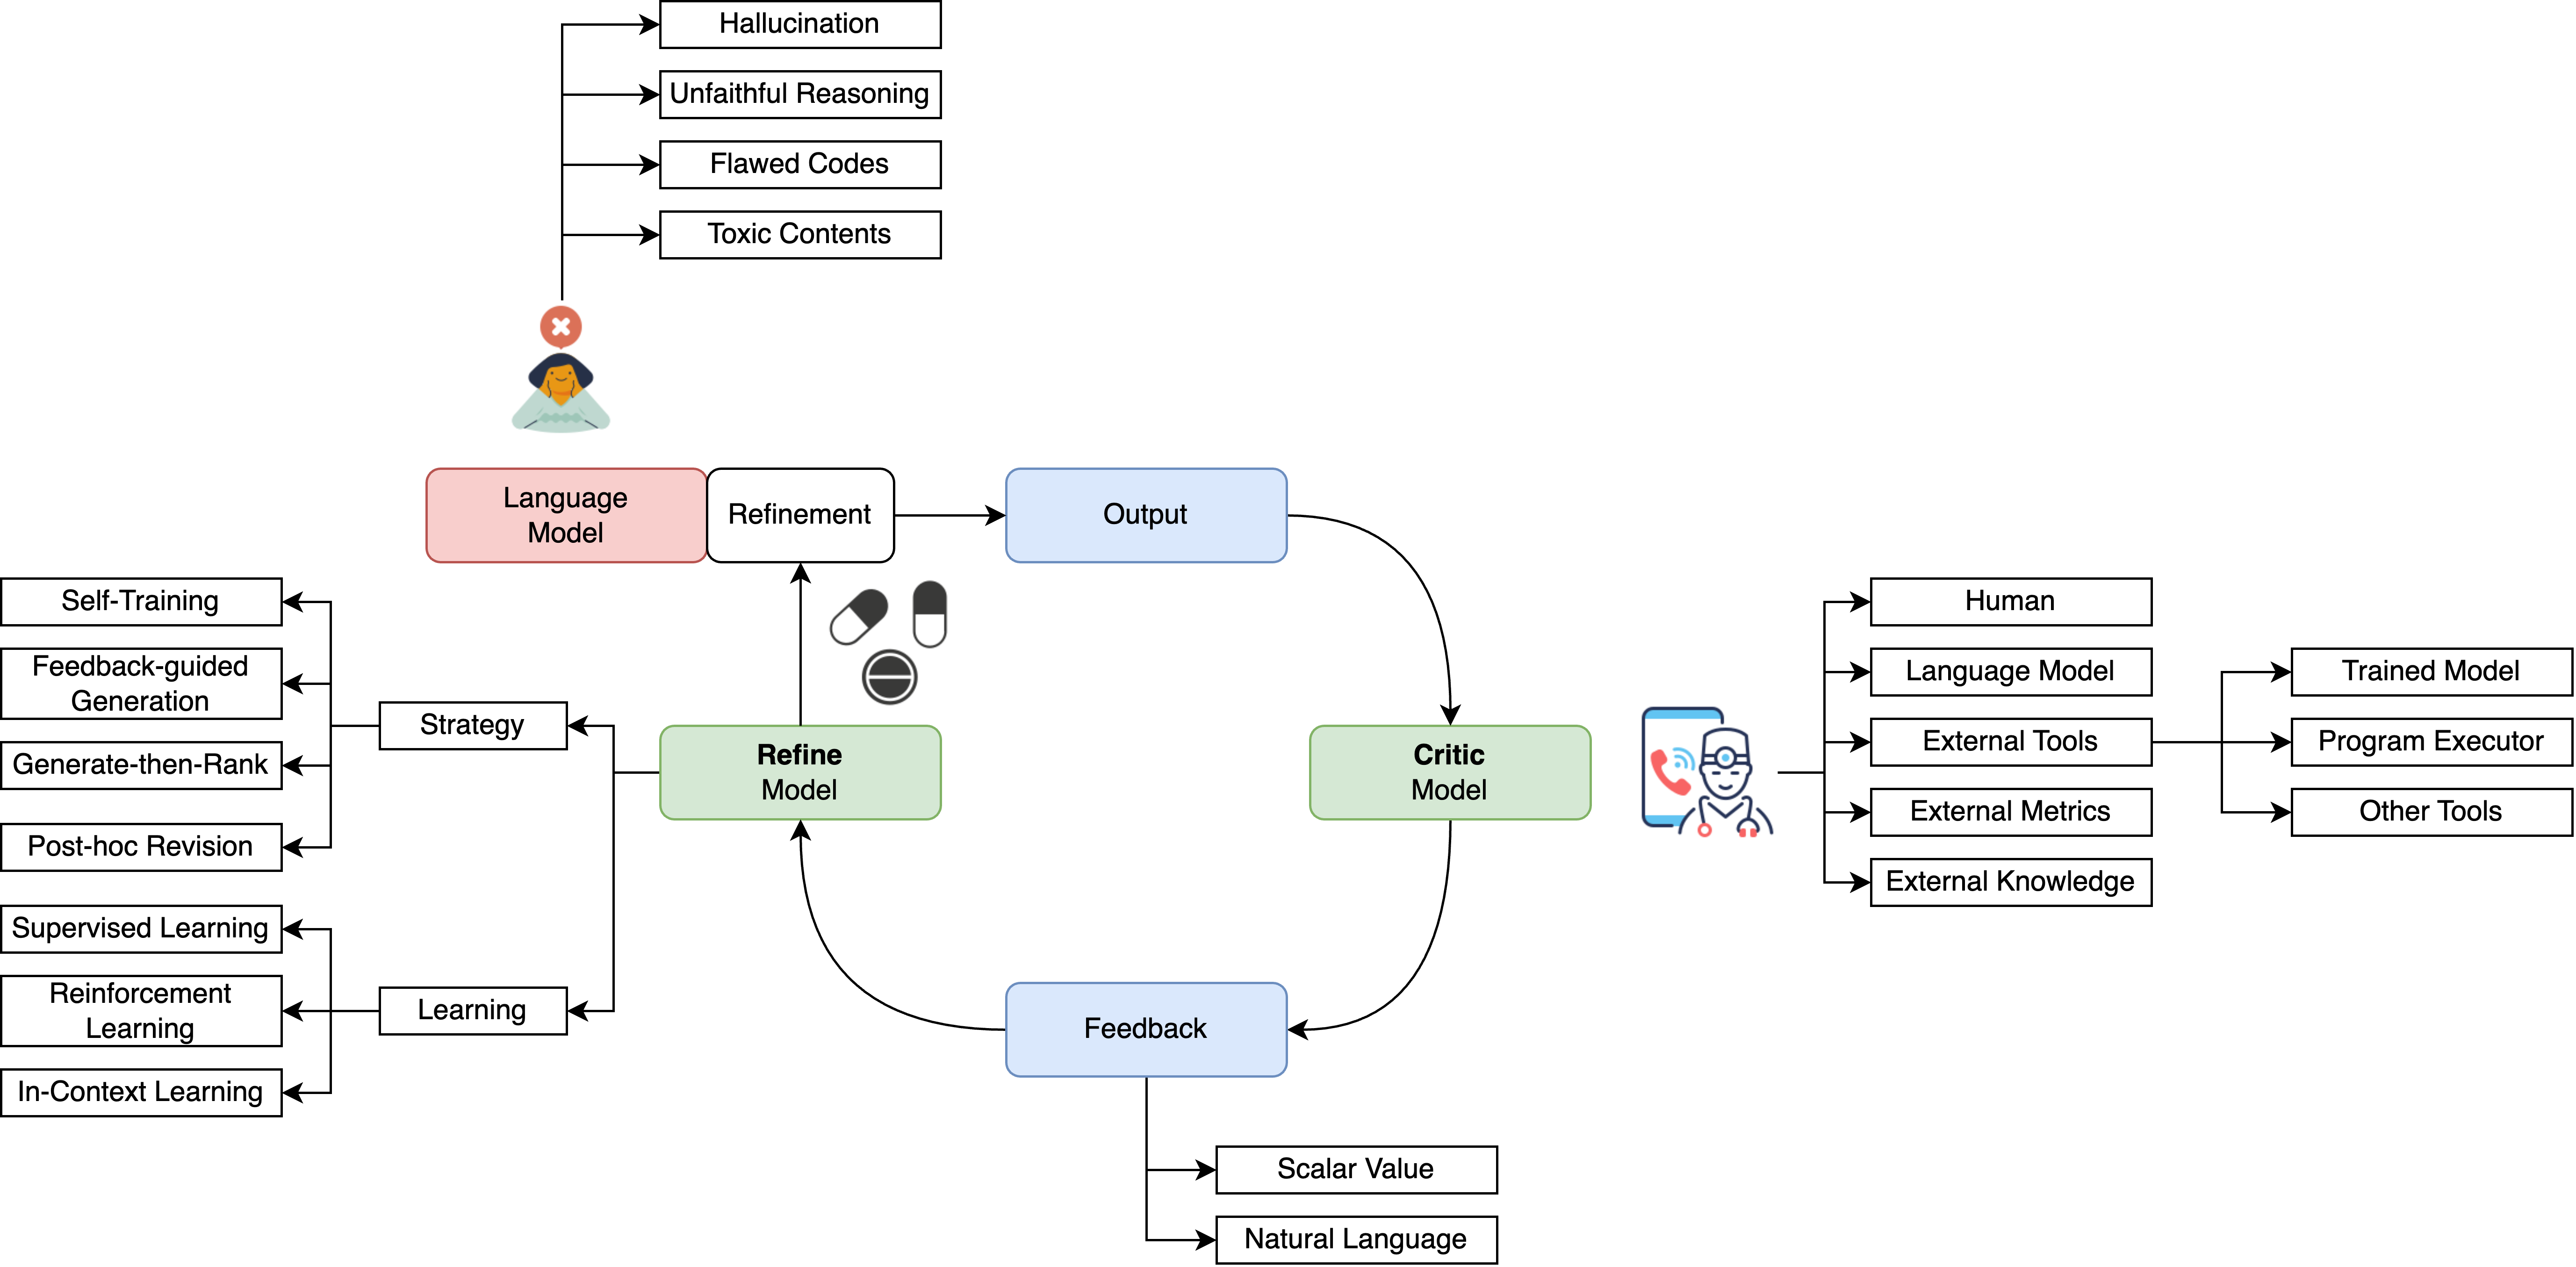
\includegraphics[scale=0.045]{img/taxonomy}
        \caption{Taxonomy of related works.}\label{fig:taxonomy}
    \end{figure}
    In Figure~\ref{fig:taxonomy}, a conceptual framework with three actors depicts related works: a \textbf{Language Model} generates initial output, a \textbf{Critic Model} analyzes and offers feedback, and a \textbf{Refine Model} adjusts either the output or the language model.
\end{frame}

\begin{frame}{Language Model}
    \begin{columns}[T]
        \begin{column}{0.70\textwidth}
            The works aimed at developing self-correcting LLMs can be classified according to the issues they tackle:
            \begin{enumerate}
                \item Hallucination: plausible-sounding but false information~\cite{gao2023rarr, zhang2023language}.

                \item Unfaithful Reasoning: derived conclusion does not follow the previously generated reasoning chain~\cite{he2022rethinking, pan2023logiclm}.

                \item Toxic Contents: content that is toxic, biased, or harmful due to biases present in the training datas~\cite{lu2022quark, gou2023critic}.

                \item Flawed Codes: flawed or incorrect code generation~\cite{chen2023teaching, olausson2023selfrepair}.
            \end{enumerate}
        \end{column}
        \begin{column}{0.30\textwidth}
            \begin{figure}[!htb]
                \centering
                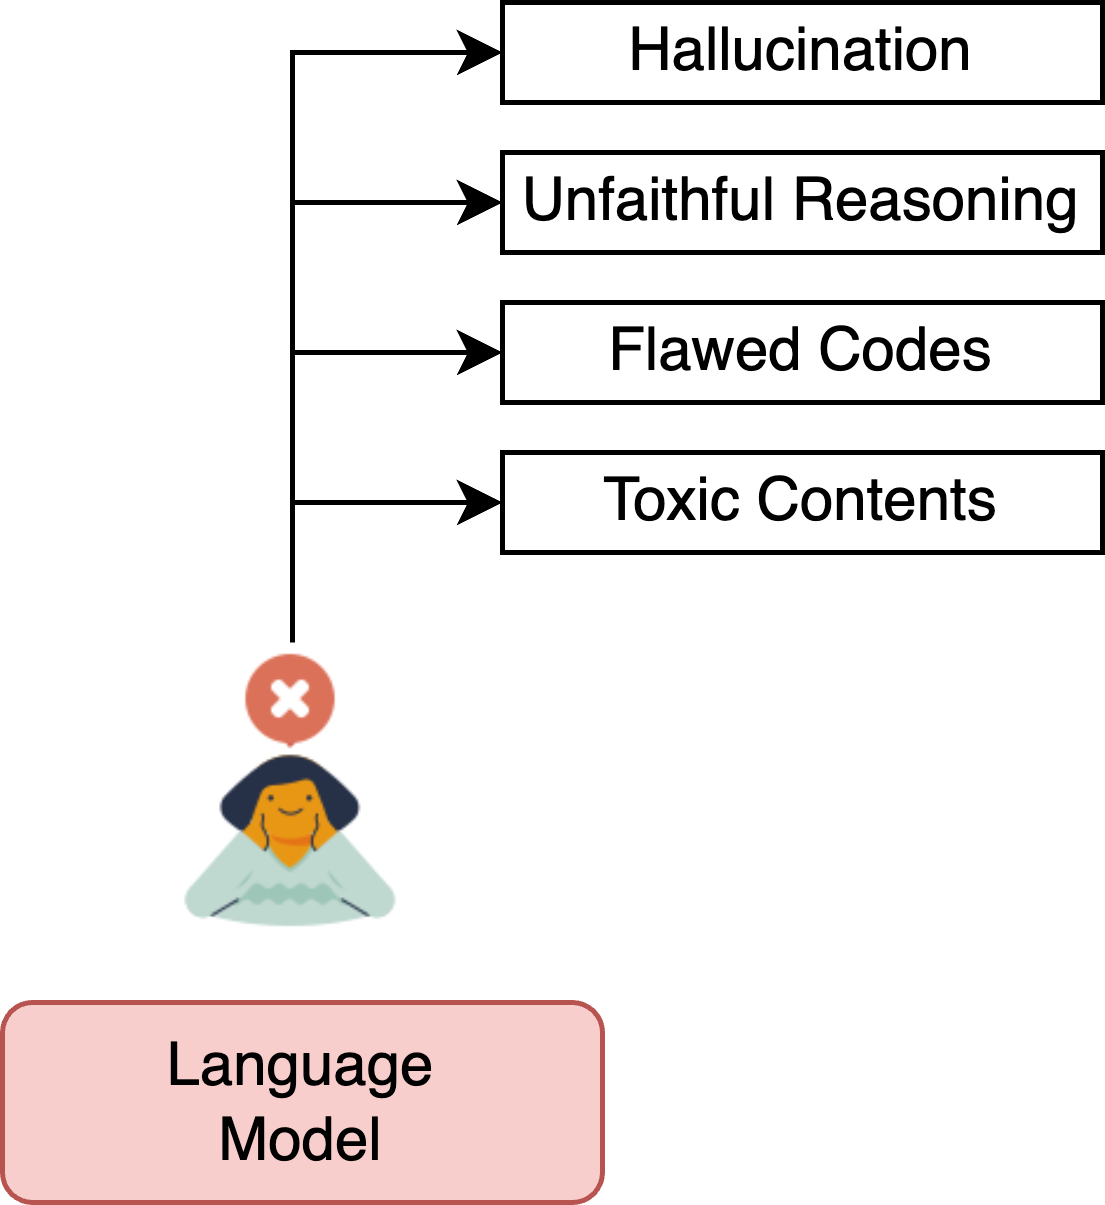
\includegraphics[scale=0.08]{img/language_model}
                \captionsetup{font=small}
                \caption{Problems of LLMs.}
            \end{figure}
        \end{column}
    \end{columns}
\end{frame}

\begin{frame}{Critic Model}
    \begin{columns}[T]
        \begin{column}{0.55\textwidth}
            Source of feedback:
            \begin{enumerate}
                \item Self-Feedback: the model itself generates feedback~\cite{weng2023large}.

                \item External Feedback: the model receives feedback from an external source (e.g., human, program executor and external knowledge)~\cite{gou2023critic}.
            \end{enumerate}

            Format of feedback:
            \begin{enumerate}
                \item Scalar Value: metrics based on pre-defined tests~\cite{weng2023large}.

                \item Natural Language: provides richer information than scalar value feedback~\cite{chen2023teaching}.
            \end{enumerate}
        \end{column}
        \begin{column}{0.45\textwidth}
            \begin{figure}[!htb]
                \centering
                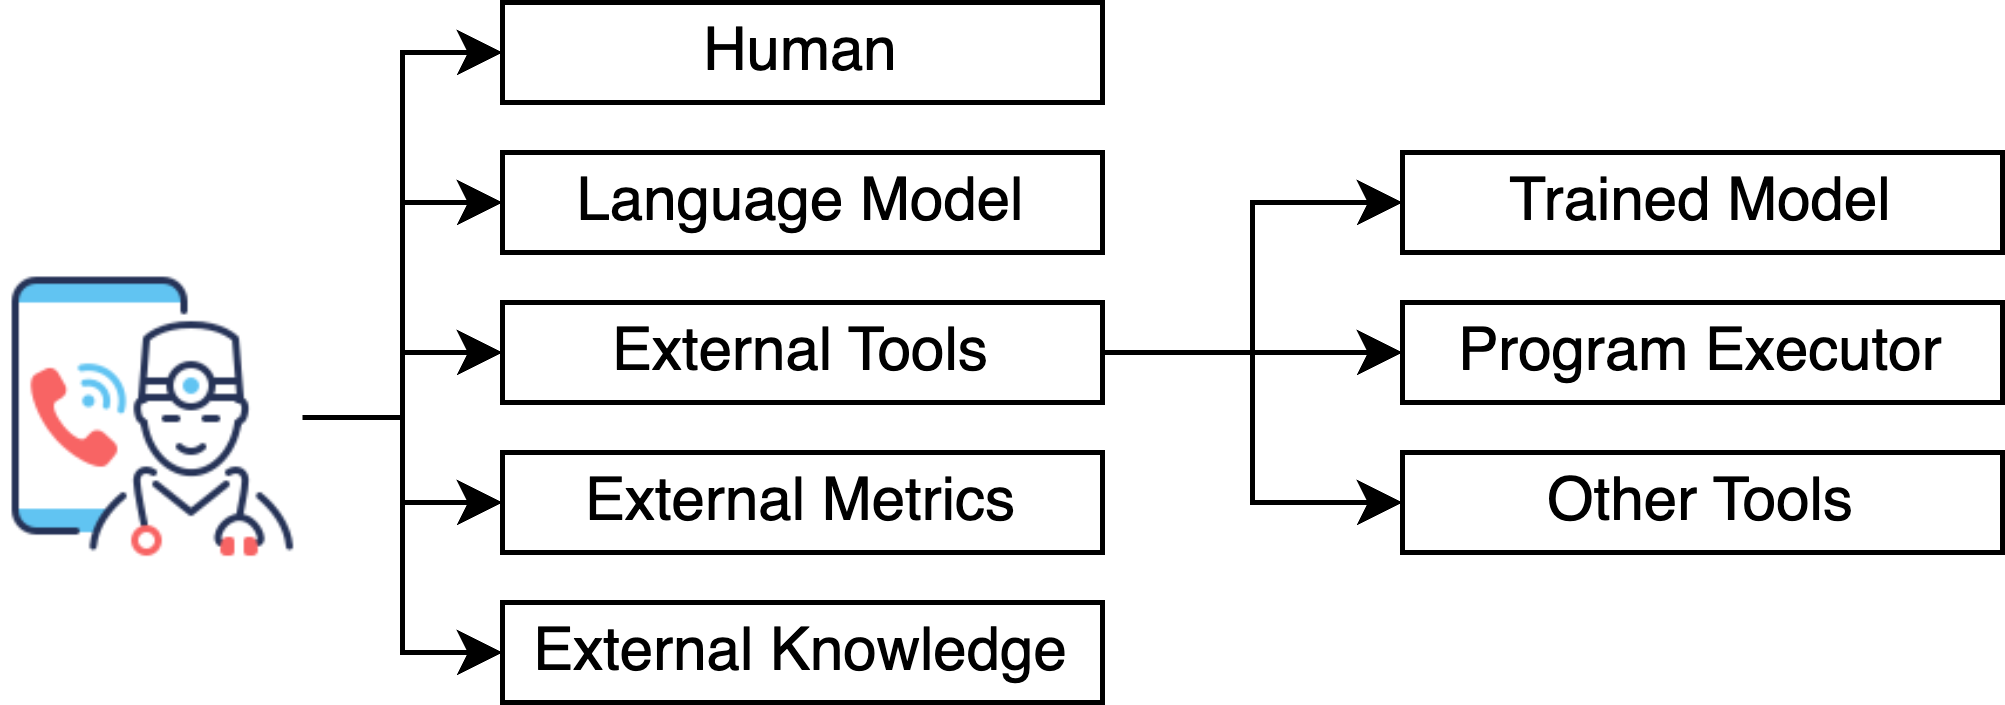
\includegraphics[scale=0.072]{img/critic_model}
                \captionsetup{font=small}
                \caption{Critic Model.}
            \end{figure}
        \end{column}
    \end{columns}
\end{frame}

\begin{frame}{Refine Model}
    The Refine Model is the most active area of research in the field. Existing works can be classified based on the following key questions:
    \begin{enumerate}
        \item Need to update the LLMs? \textbf{Yes}: Self-Training~\cite{huang2022large}, Supervised Learning~\cite{bai2022training}, Reinforcement Learning~\cite{dubois2024alpacafarm}, In-Context Learning~\cite{dong2022survey}.

        \item When to refine: generation-time or post-hoc?
              \begin{itemize}
                  \item Generation-time: Generate-then-Rank~\cite{cobbe2021training}, Feedback-Guided Generation~\cite{yao2023tree}.
                  \item Post-hoc: Models/Tools as Feedback~\cite{zhang2023selfedit}, Multi-Agent Debate~\cite{du2023improving}.
              \end{itemize}
    \end{enumerate}
\end{frame}

\section{Methodology}

\begin{frame}{Chain-of-Thought Prompting}
    \textit{Chain-of-Thought} (CoT) prompting~\cite{wei2023chainofthought}, which uses a series of intermediate reasoning steps, significantly improves the ability of LLMs to perform complex reasoning.\\
    \begin{figure}[!htb]
        \centering
        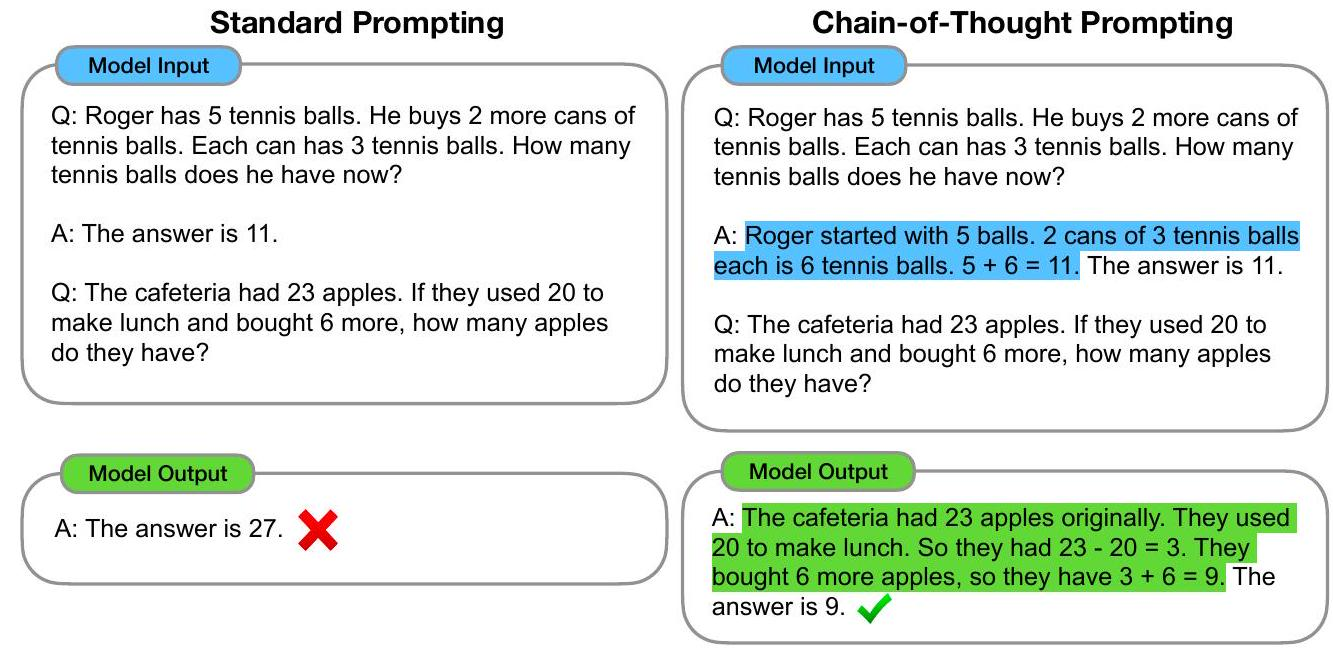
\includegraphics[width=0.75\textwidth]{img/cot_prompting}
        \captionsetup{font=small,labelformat=empty}
        \caption{Chain-of-Thought reasoning processes are highlighted.}
    \end{figure}
\end{frame}

\begin{frame}{CoT Techniques}
    \begin{figure}[!htb]
        \centering
        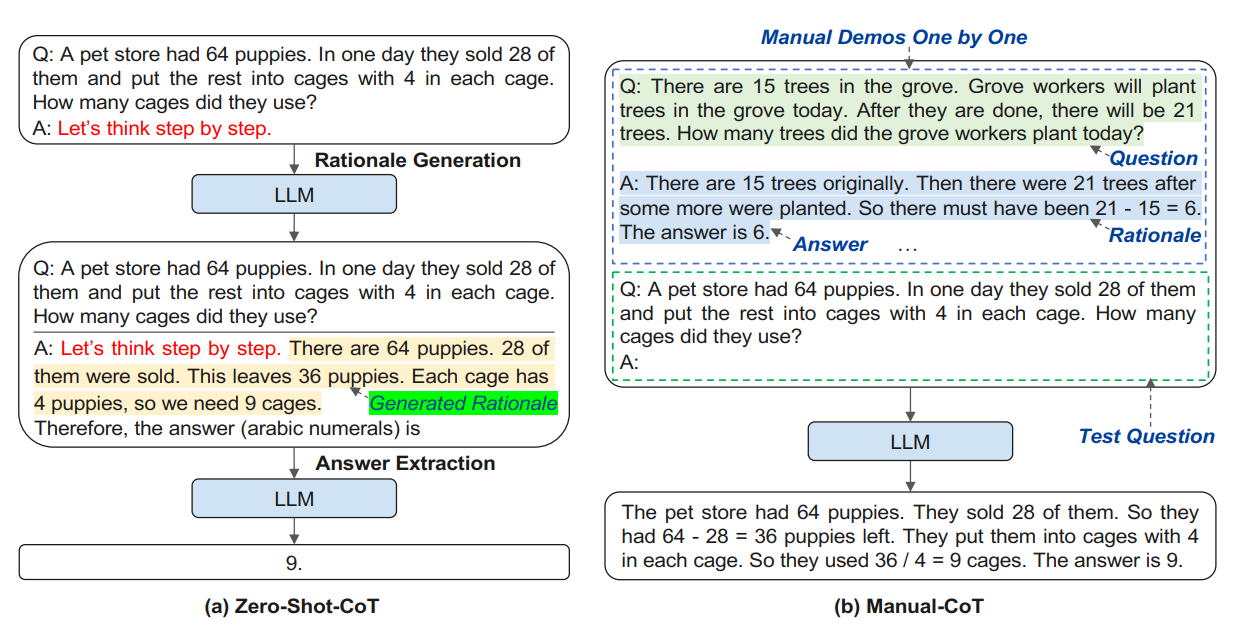
\includegraphics[width=\textwidth]{img/cot_types}
        \captionsetup{font=small,labelformat=empty}
        \caption{Zero-shot-CoT vs. Manual-CoT.}
    \end{figure}
\end{frame}

\begin{frame}{CoT Techniques}
    An automatic CoT prompting method (Auto-CoT~\cite{zhang2022automatic}), generates diverse samples and reasoning chains. In ten GPT-3 benchmark reasoning tasks, it consistently meets or surpasses manual CoT performance.
    \begin{figure}[!htb]
        \centering
        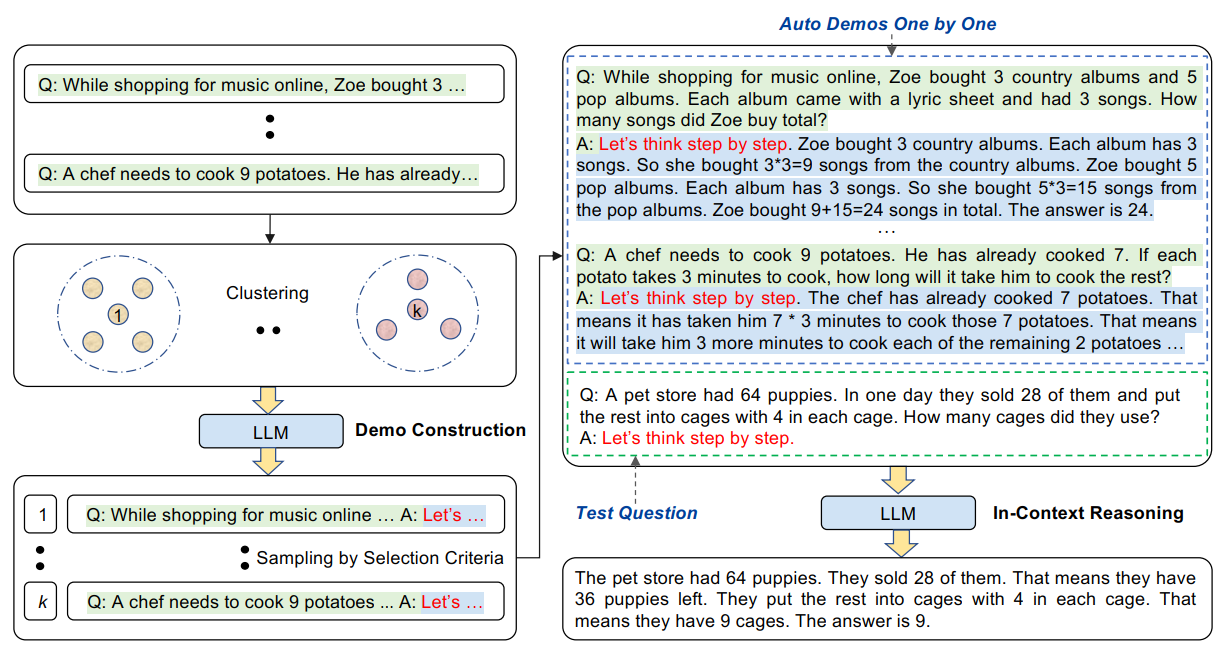
\includegraphics[width=0.85\textwidth]{img/auto_cot}
        \captionsetup{font=small,labelformat=empty}
        \caption{Auto-CoT.}
    \end{figure}
\end{frame}

\begin{frame}{CoT-SelfEvolve Architecture}
    \begin{figure}[!htb]
        \centering
        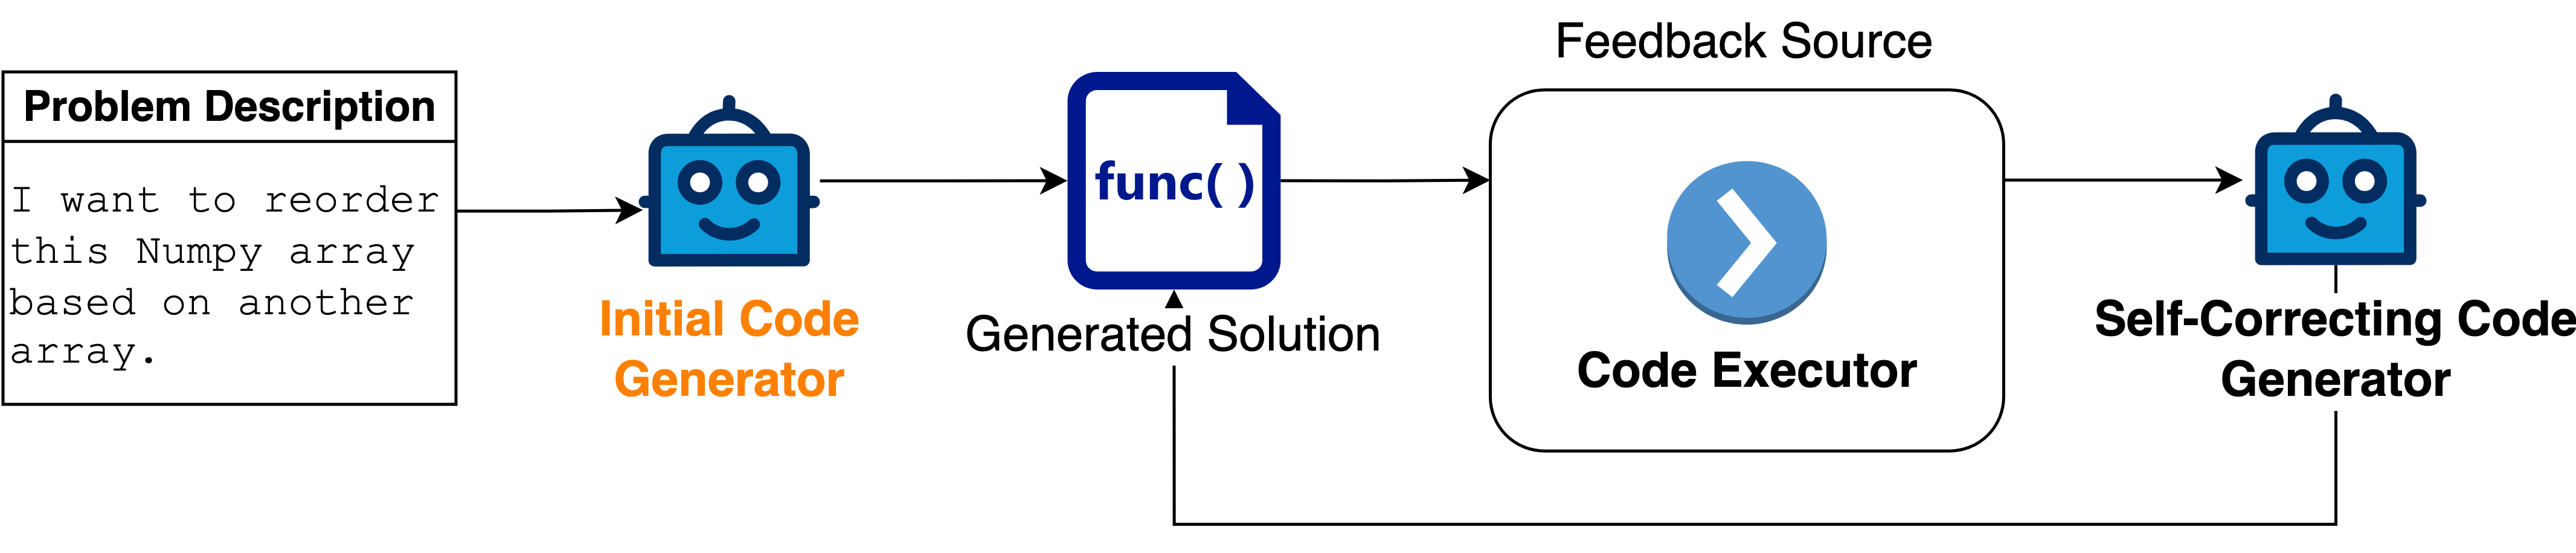
\includegraphics[width=0.70\textwidth]{img/selfevolve_architecture}
        \captionsetup{font=small,labelformat=empty}
        \caption{Architecture of the SelfEvolve~\cite{jiang2023selfevolve} model.}
    \end{figure}
    \begin{figure}[!htb]
        \centering
        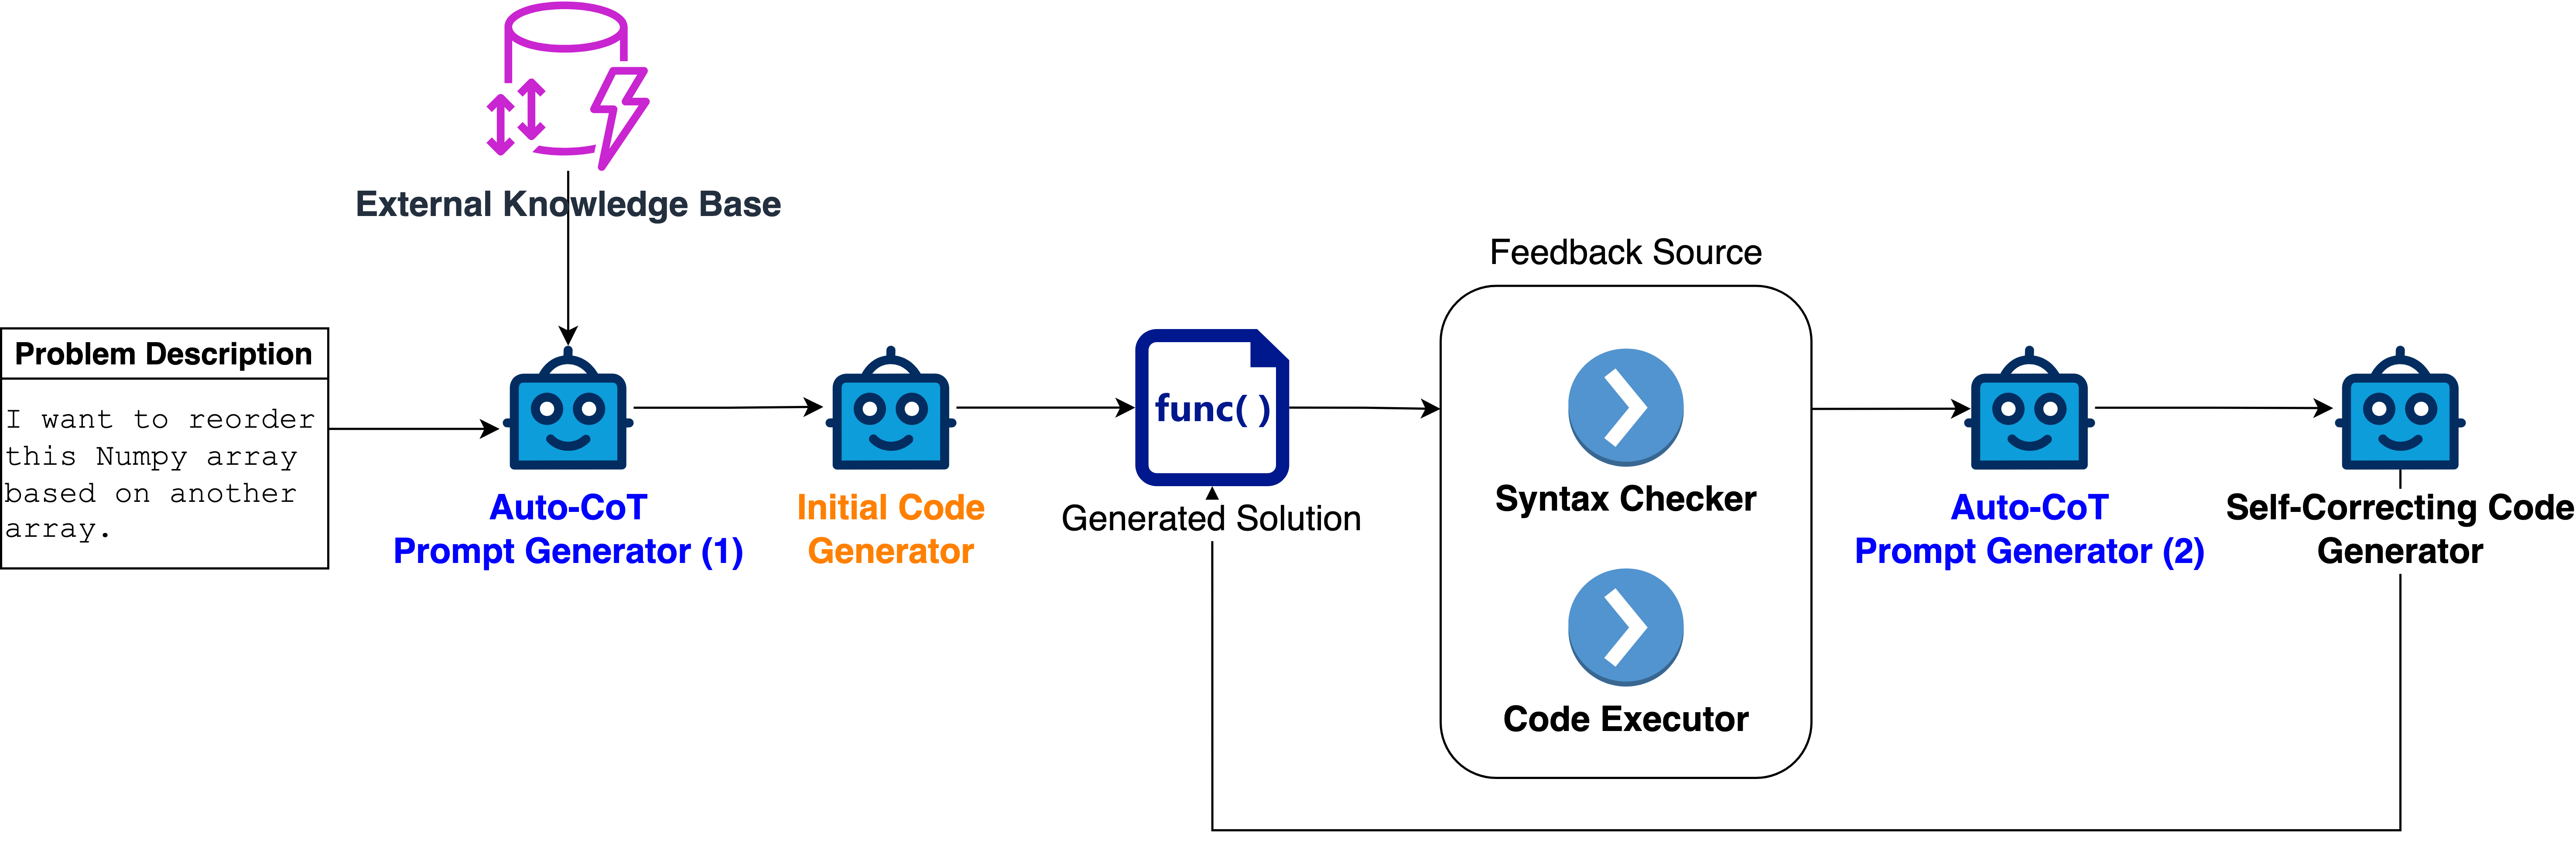
\includegraphics[width=0.90\textwidth]{img/cot_selfevolve_architecture}
        \captionsetup{font=small,labelformat=empty}
        \caption{Architecture of the CoT-SelfEvolve model (this study).}
    \end{figure}
\end{frame}

\begin{frame}{Auto-CoT Prompt Generation (1)}
    The initial Auto-CoT prompt generator integrates problem descriptions with relevant StackOverflow discussions. This in-context material aids a LLM in reasoning and hint generation for problem-solving. These hints then serve as CoT prompts for another LLM (Code Generator).
    \begin{figure}[!htb]
        \centering
        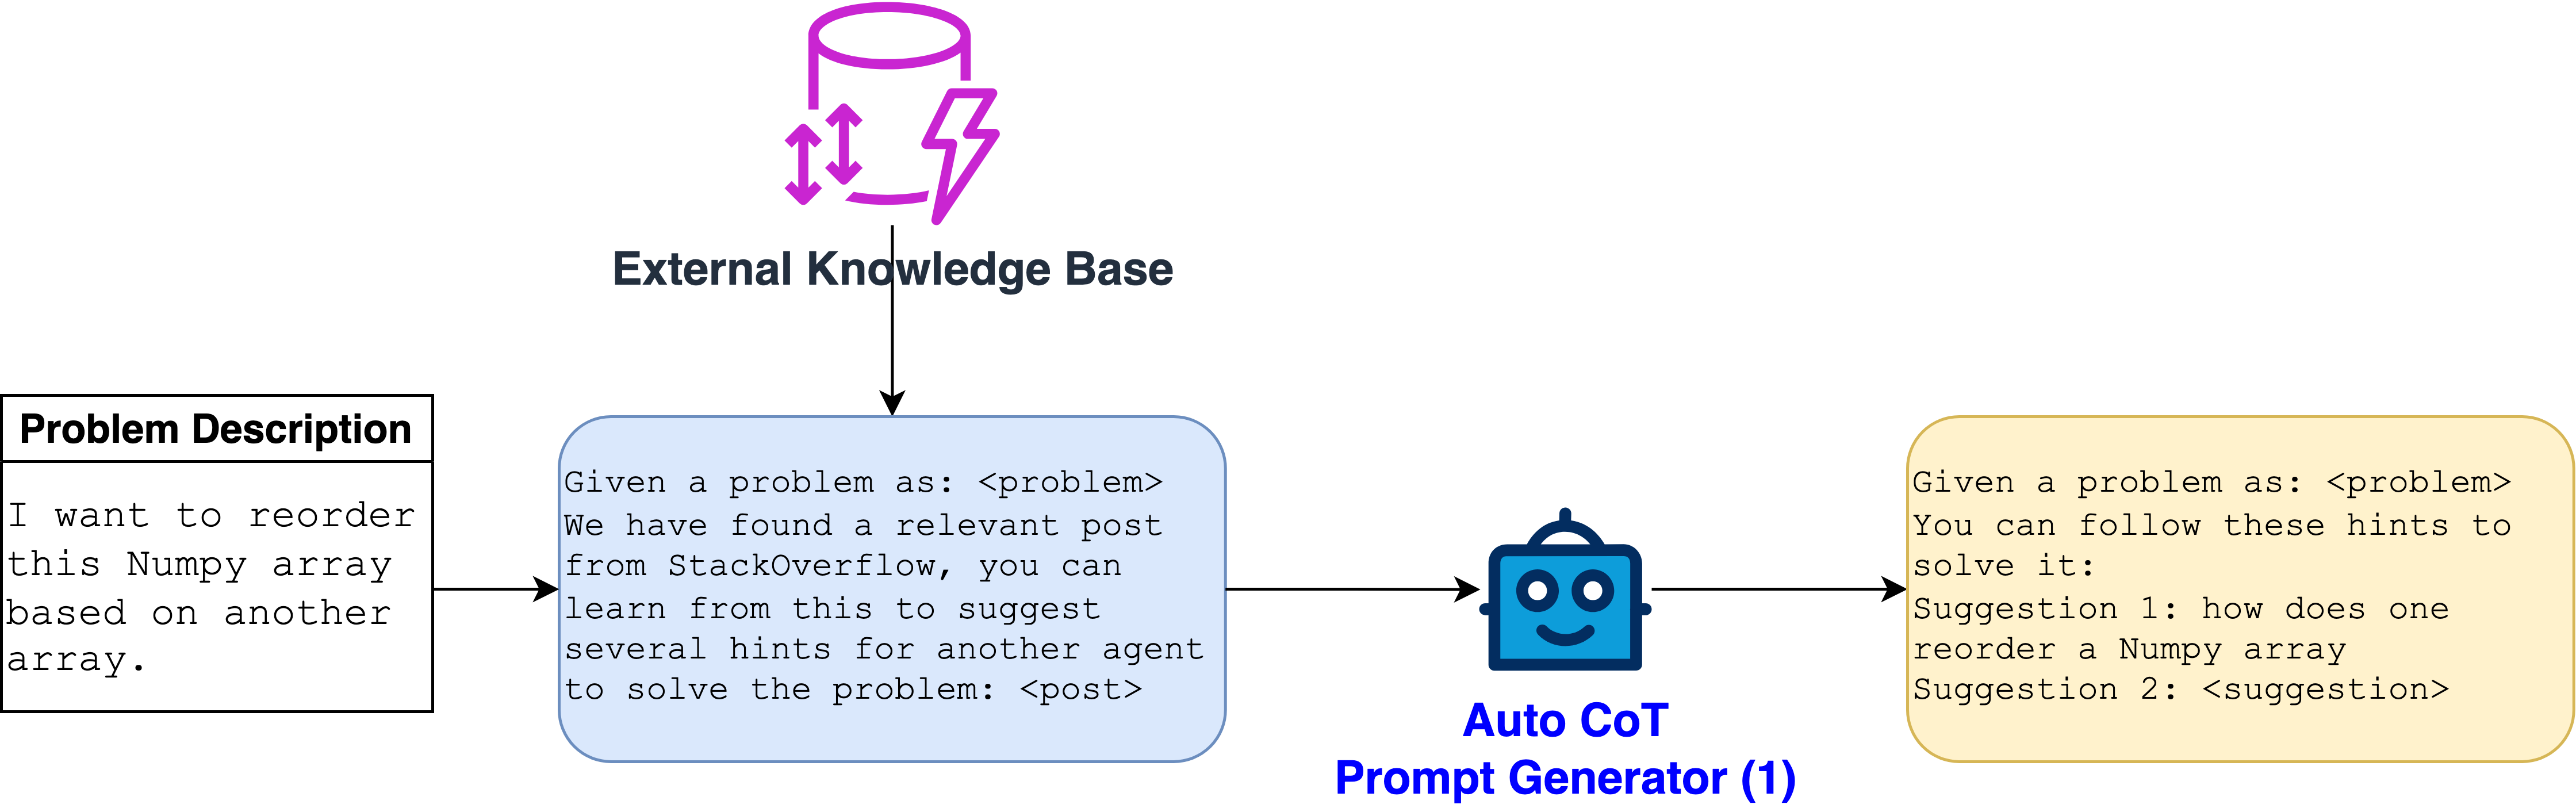
\includegraphics[width=\textwidth]{img/cot_generator_1}
        \captionsetup{font=small,labelformat=empty}
        \caption{Auto-CoT Prompt Generation (1).}
    \end{figure}
\end{frame}

\begin{frame}{Auto-CoT Prompt Generation (2)}
    The second Auto-CoT prompt generator combines problem descriptions with feedback from syntax checkers or code executors. It aims to generate self-reflective questions for a LLM to consider during problem-solving.
    \begin{figure}[!htb]
        \centering
        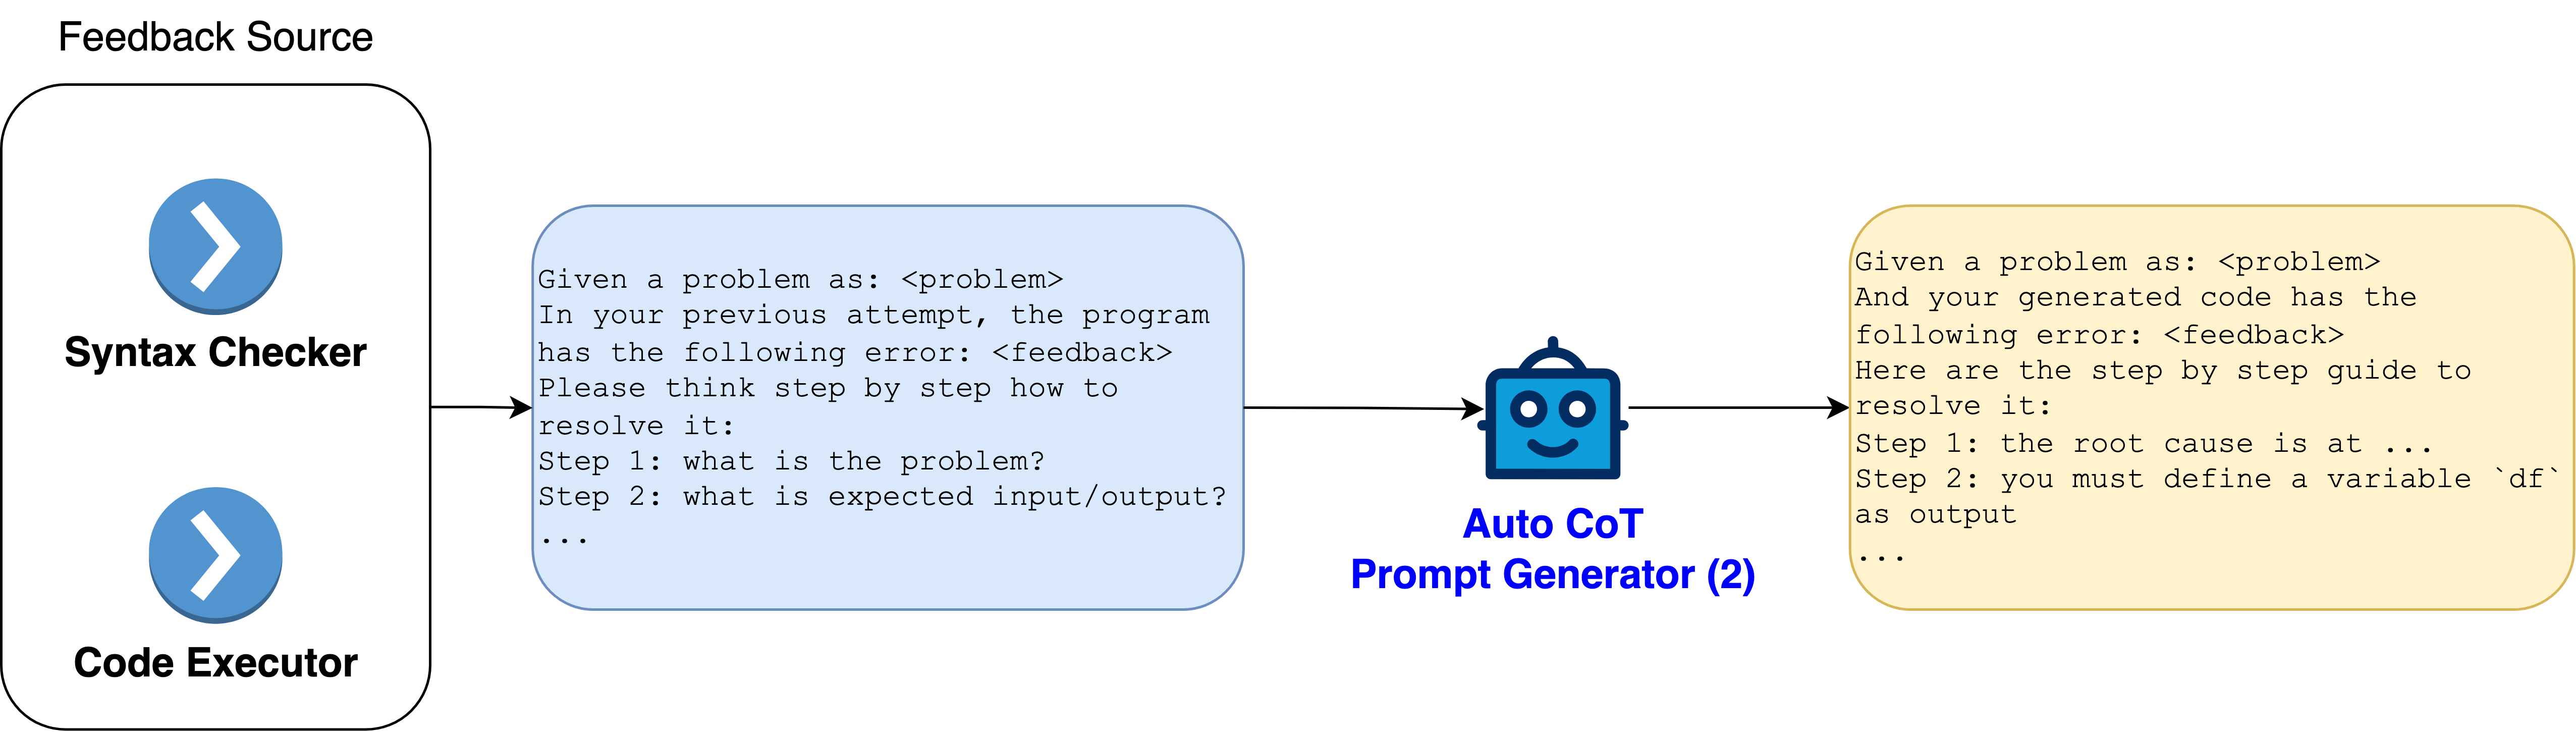
\includegraphics[width=\textwidth]{img/cot_generator_2}
        \captionsetup{font=small,labelformat=empty}
        \caption{Auto-CoT Prompt Generation (2).}
    \end{figure}
\end{frame}

\begin{frame}{External Knowledge Base}
    \begin{columns}[T] % align columns
        \begin{column}{.4\textwidth}
            \begin{figure}[!htb]
                \centering
                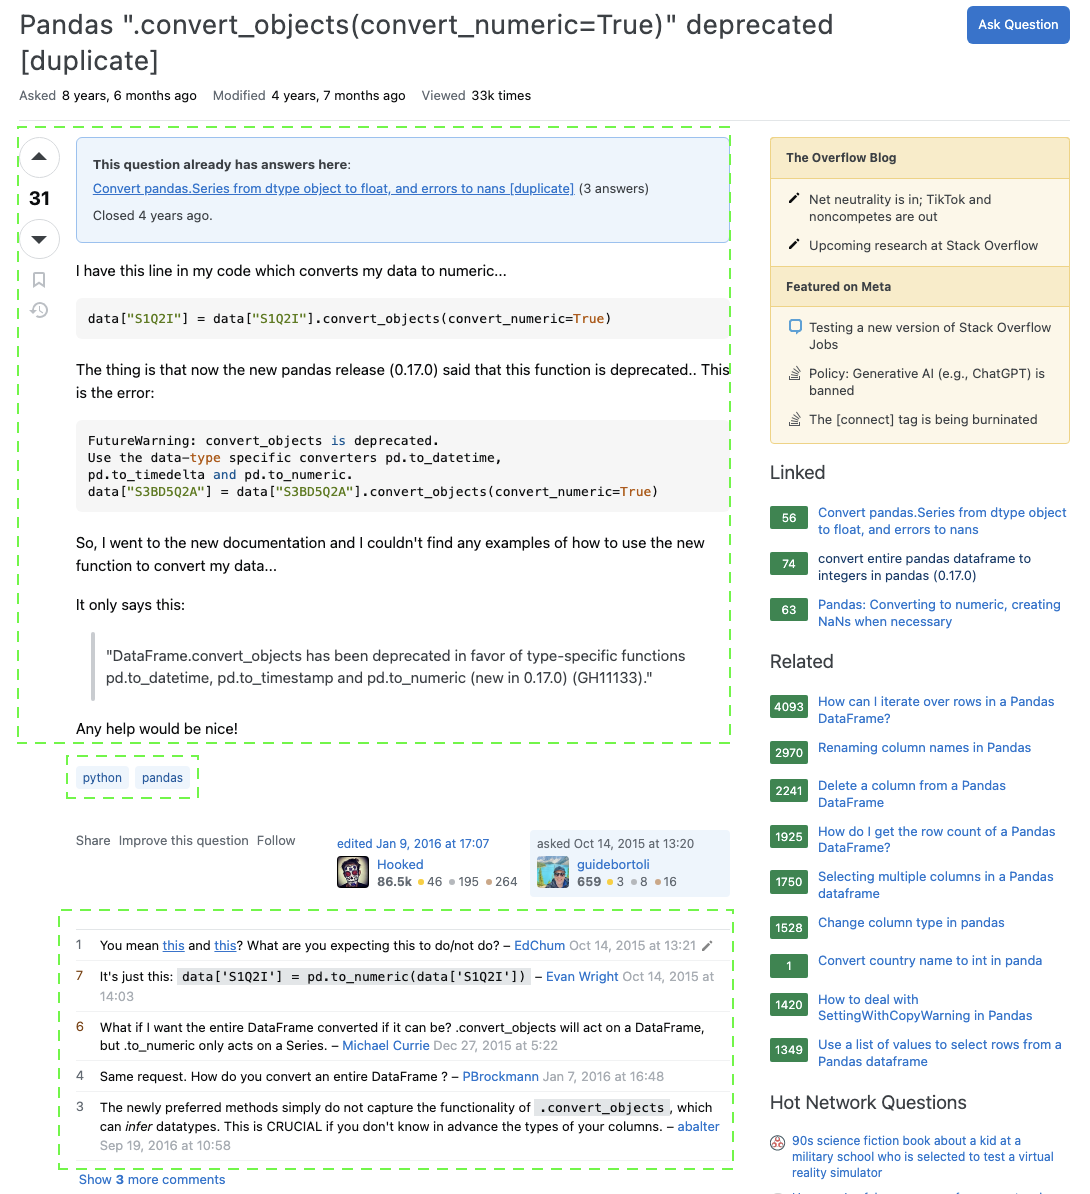
\includegraphics[width=\textwidth]{img/stackoverflow.png}
                \captionsetup{font=small,labelformat=empty}
                \caption{Example of StackOverflow discussions.}
            \end{figure}
        \end{column}%
        \begin{column}{.6\textwidth}
            \begin{itemize}
                \item An external knowledge base, narrowed to seven Python libraries, is constructed from 500,000 StackOverflow discussions.
                \item Each document amalgamates a problem description with its comments.
                \item OpenAI's text-embedding-ada-02 model generates the embeddings.
                \item Using the HNSW algorithm on top of these embeddings to retrieve relevant documents for a specific problem.
            \end{itemize}
        \end{column}%
    \end{columns}
\end{frame}

\section{Objective and Scope}

\begin{frame}{Objective}
    \begin{enumerate}
        \item Comprehensively review self-correcting LLMs for software debugging.

        \item Investigate instructing LLMs to optimally resolve bugs, improving on published methods.

        \item Identify evaluation benchmarks.

        \item Implement a Chain-of-Thought prompting and modular code analysis model, and researching improvements.

        \item Comparatively evaluate results against published methods.
    \end{enumerate}
\end{frame}

\begin{frame}{Scope}
    \begin{enumerate}
        \item Focus on self-correction techniques in LLMs for Python data science error debugging.

        \item Use the DS-1000~\cite{pmlr-v202-lai23b} dataset of Python data science bugs.

        \item Utilize Azure OpenAI ChatGPT Turbo 3.5 LLM.

        \item Develop a Chain-of-Thought prompting and modular code analysis system to effectively resolve bugs.
    \end{enumerate}
\end{frame}

\begin{frame}{Dataset}
    1000 Python data science coding problems, each with:
    \begin{block}{Problem Description}
        \small
        Problem:
        How do I get the dimensions of an array? For instance, this is (2, 2):\\
        a = np.array([[1,2],[3,4]])
    \end{block}

    \begin{columns}[T]
        \begin{column}{0.50\textwidth}
            \begin{block}{Buggy Code}
                \small
                <code>\\
                import numpy as np\\
                a = np.array([[1,2],[3,4]])\\
                </code>\\
                result = $\ldots$ \# put solution in this variable\\
                BEGIN SOLUTION\\
                <code>
            \end{block}
        \end{column}
        \begin{column}{0.45\textwidth}
            \begin{block}{Unit Test}
                \small
                def test(result, ans):\\
                \ \ \ \ assert\_array\_equal(result, ans)\\
                \ \ \ \ return 1
            \end{block}
        \end{column}
    \end{columns}
\end{frame}


\section{Progress}

\begin{frame}{Overall Design}
    \begin{figure}[!htb]
        \centering
        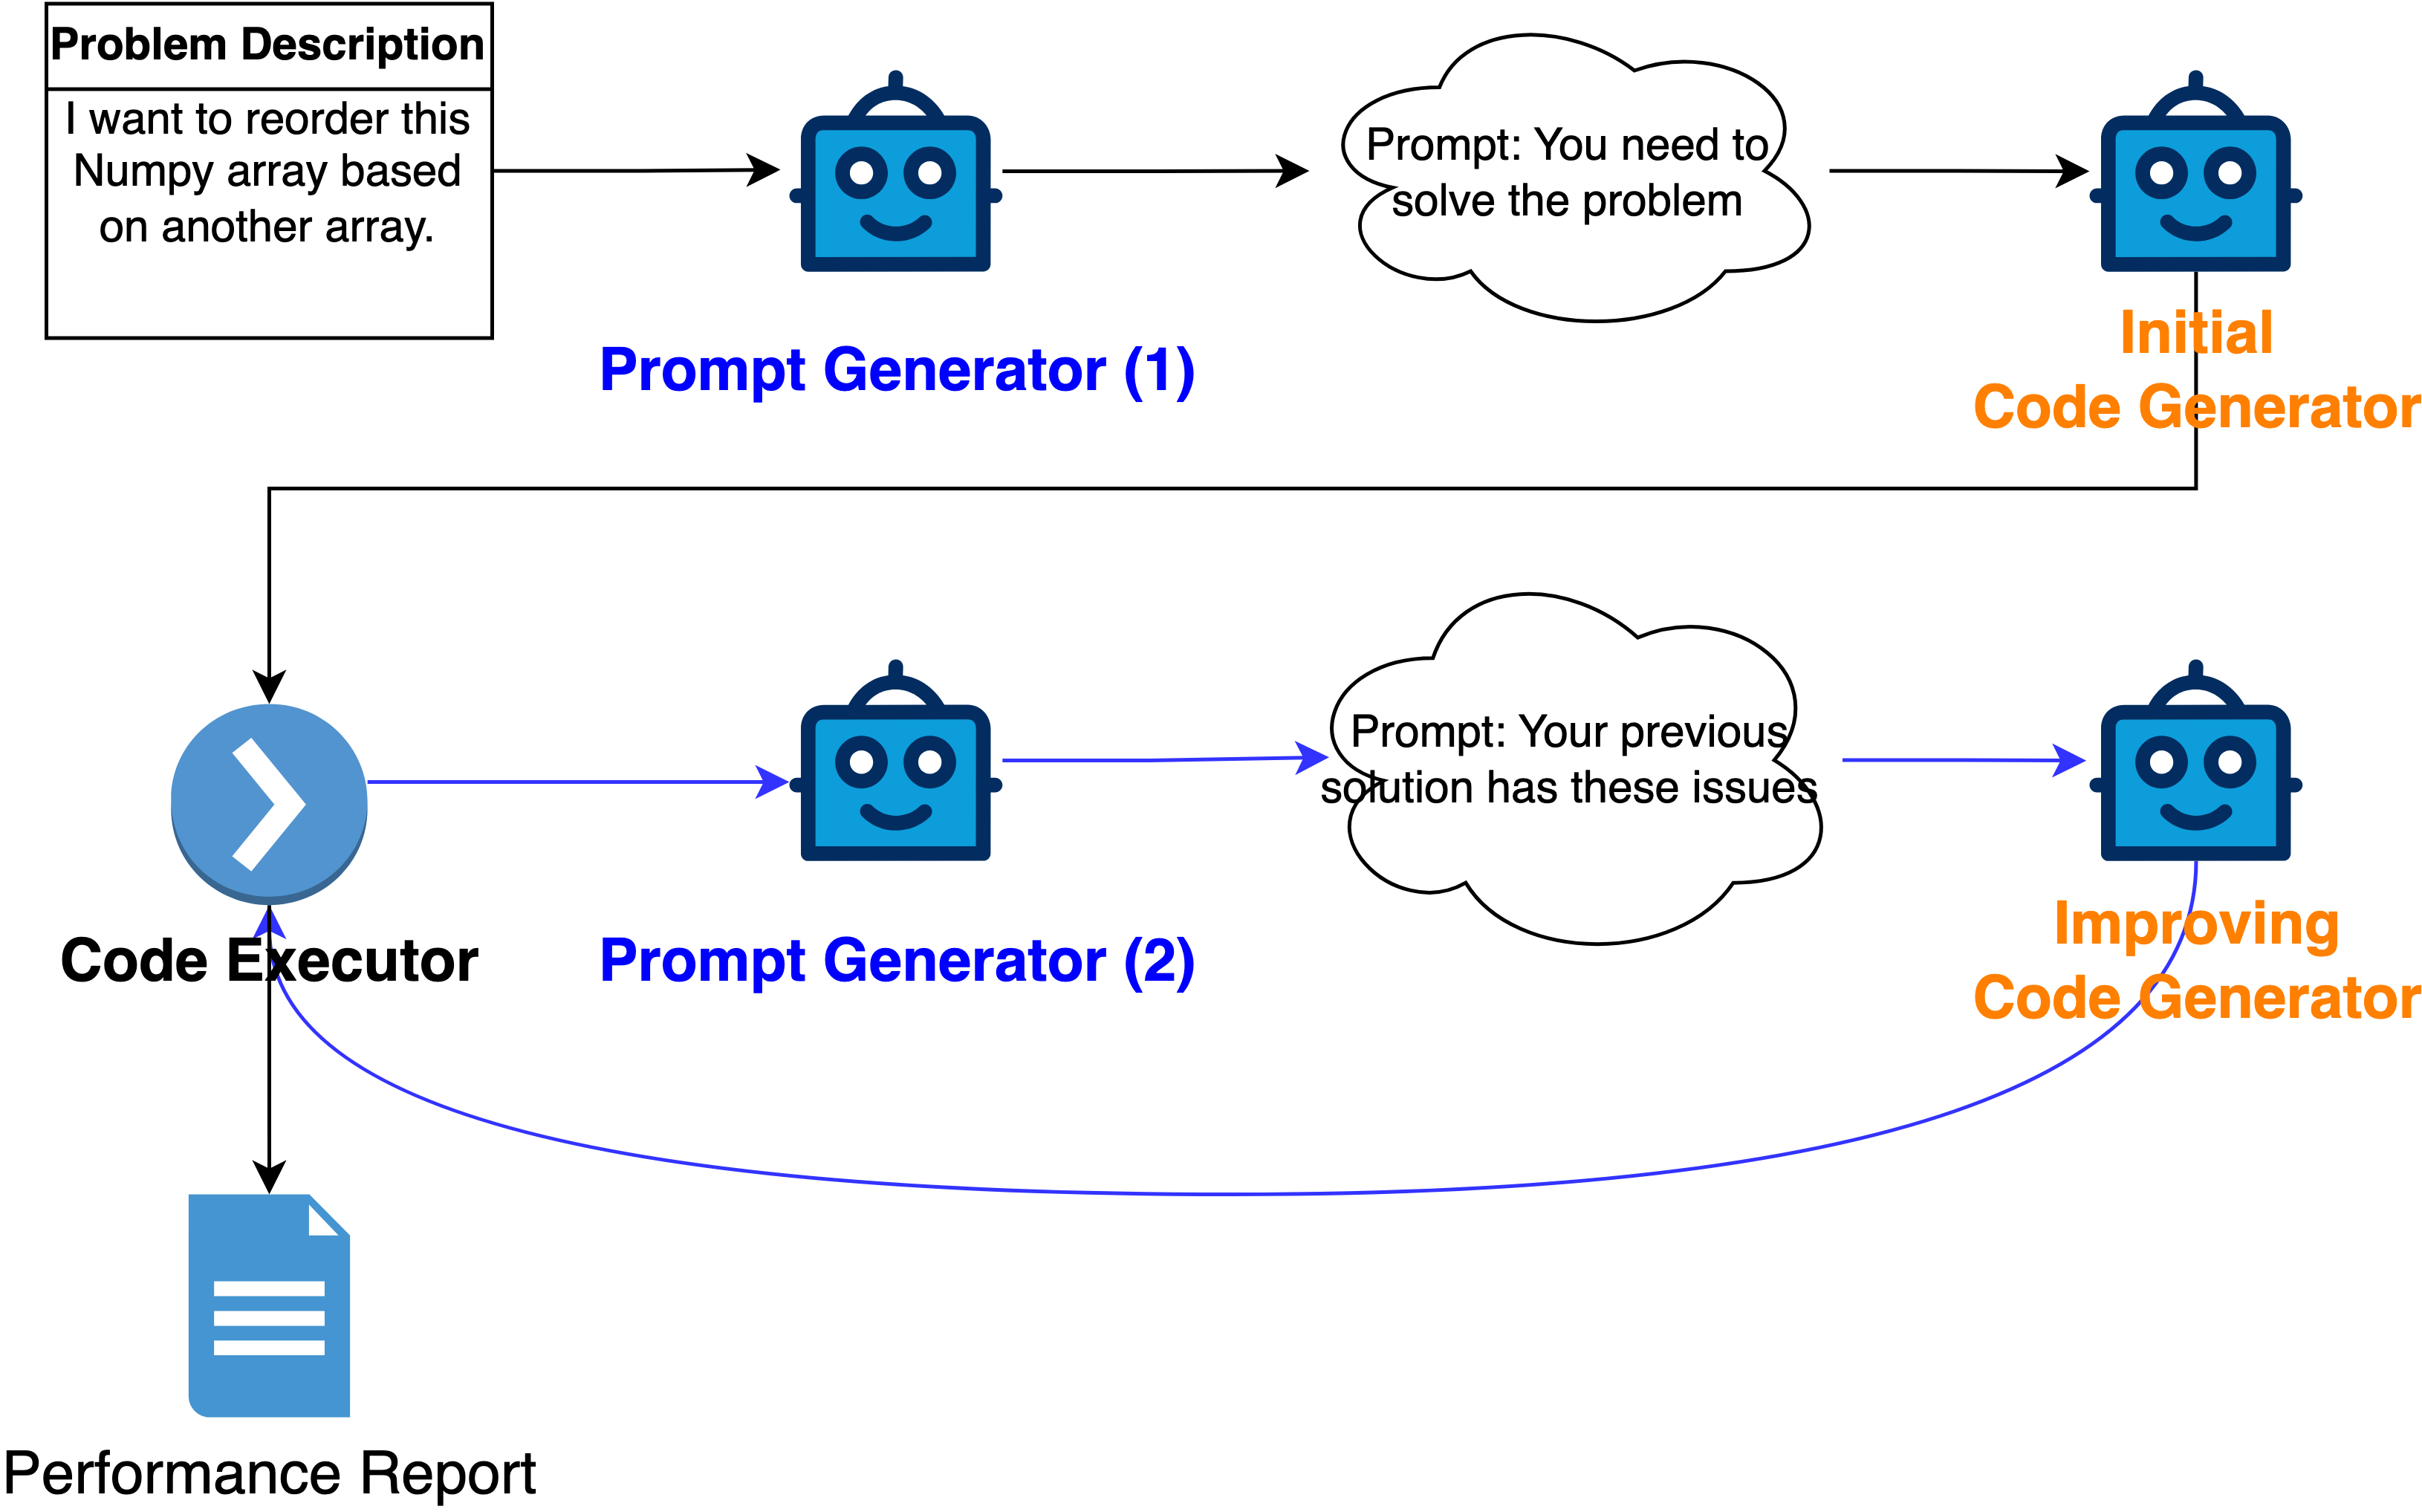
\includegraphics[width=0.9\textwidth]{img/selfdebug_design}
        \captionsetup{font=small,labelformat=empty}
        \caption{The modules of the proposed system.}
    \end{figure}
\end{frame}

\begin{frame}{Progress Update \: 08 Mar 2024}
    Completed:
    \begin{itemize}
        \item Prompt Generator (1) with Zero-shot prompts (baseline)
        \item Initial-Code Generator with ChatGPT 3.5 API
        \item Code Executor on Virtual environment to run test cases
        \item Performance Report using accuracy score
    \end{itemize}

    Baseline Results:
    \begin{tabular}{lr}
        Library    & Accuracy \\
        \hline
        Matplotlib & 18.06\%  \\
        Scipy      & 16.04\%  \\
        Pandas     & 8.93\%   \\
        Numpy      & 5.91\%   \\
        Sklearn    & 9.57\%   \\
        Tensorflow & 17.78\%  \\
        Pytorch    & 2.94\%   \\
    \end{tabular}
\end{frame}

\begin{frame}{Progress Update \: 08 Mar 2024}
    Next Steps:
    \begin{itemize}
        \item Prompt Generator (2) with CoT prompts based on code execution feedback
        \item Correcting-Code Generator
    \end{itemize}
\end{frame}

\begin{frame}{Progress Update \: 29 Mar 2024}
    Completed:
    \begin{itemize}
        \item Prompt Generator (1) with CoT prompts
        \item Prompt Generator (2) with direct feedback from code execution
        \item Correcting-Code Generator
    \end{itemize}

    Improved Results:
    \begin{tabular}{lr}
        Library    & Accuracy \\
        \hline
        Matplotlib & 41.94\%  \\
        Scipy      & 16.98\%  \\
        Pandas     & 23.71\%  \\
        Numpy      & 15.91\%  \\
        Sklearn    & 41.74\%  \\
        Tensorflow & 28.89\%  \\
        Pytorch    & 38.24\%  \\
    \end{tabular}
\end{frame}

\begin{frame}{Progress Update \: 29 Mar 2024}
    Example of CoT prompt:

    Here are some step-by-step suggestions to help solve the problem:

    1. \textbf{Suggestion 1}: First, let's understand the problem. The goal is to shuffle the order of the DataFrame's rows according to a given list. The list represents the desired order of the rows.

    2. \textbf{Suggestion 2}: To achieve this, we can use the `iloc' function in pandas to select the rows of the DataFrame based on the given list. The `iloc' function allows us to select rows by their integer position.

    3. \textbf{Suggestion 3}: Start by creating a new DataFrame that contains the shuffled rows. You can do this by using the `iloc' function with the given list as the index. For example, `shuffled\_df = df.iloc[List]`.

    4. \textbf{Suggestion 4}: Finally, assign the shuffled DataFrame to the `result' variable. This will be the solution to the problem. For example, `result = shuffled\_df`.
\end{frame}

\begin{frame}{Progress Update \: 29 Mar 2024}
    Next Steps:
    \begin{itemize}
        \item Analyze the failed test cases to improve the Prompt Generator (2)
        \item Connect with more LLMs: Claude 2.0, GPT-4, etc.
    \end{itemize}
\end{frame}


\section{Demo}

\begin{frame}{Demo}
    \begin{columns}[T]
        \begin{column}{0.5\textwidth}
            The demo code on GitHub at this \href{https://github.com/tqtensor/wolverine}{link}.\\
            In this example there are two bugs:
            \begin{enumerate}
                \item `subtract\_number' function is not defined.

                \item The return must be `result'.
            \end{enumerate}
        \end{column}
        \begin{column}{0.5\textwidth}
            \begin{figure}[!htb]
                \centering
                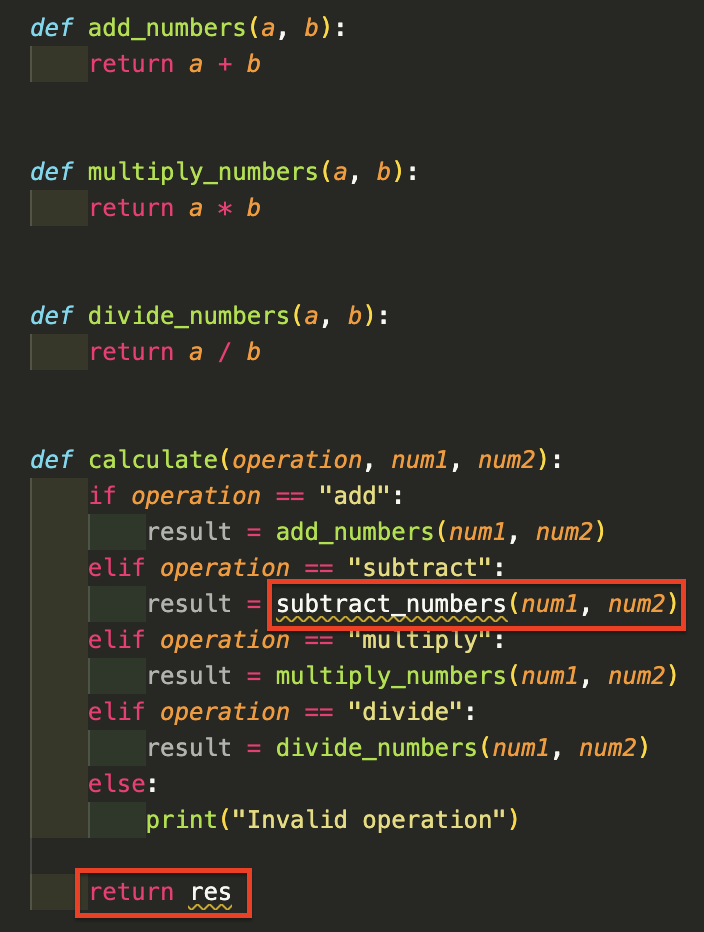
\includegraphics[width=0.7\textwidth]{img/demo}
                \captionsetup{font=small,labelformat=empty}
                \caption{Example of Python bug.}
            \end{figure}
        \end{column}
    \end{columns}
\end{frame}


\begin{frame}{Q\&A}
    \begin{figure}[!htb]
        \centering
        
\includegraphics[scale=1]{img/qna}
    \end{figure}
\end{frame}

\begin{frame}
    \begin{center}
        \Huge Thank you for your attention!
    \end{center}
\end{frame}

\begin{frame}[allowframebreaks]{References}
    \bibliography{references}
\end{frame}

\end{document}
